\documentclass{article}

% For visualization.
\usepackage{graphicx} 

% For citations
\usepackage[authoryear,round]{natbib}

% For algorithms
\usepackage{amsmath}
\usepackage{amsthm}
\usepackage{authblk}

\hyphenation{general-iza-tions}
\hyphenation{distri-bution}
\hyphenation{Zel-ter-man}

\newtheorem{lemma}{Lemma}
\newtheorem{corollary}{Corollary}
\newtheorem{prop}{Proposition}

\begin{document}

\title{SNB Results Paper 2}

\author[1]{Michael J. Kane}
\author[1]{Daniel Zelterman}

\affil[1]{Department of Biostatistics, Yale University, New Haven CT, USA}

\maketitle

\begin{abstract}
This paper other properties of the snb...
\end{abstract}

\section{Introduce the Z-Plot Construction}

\begin{figure}[ht]
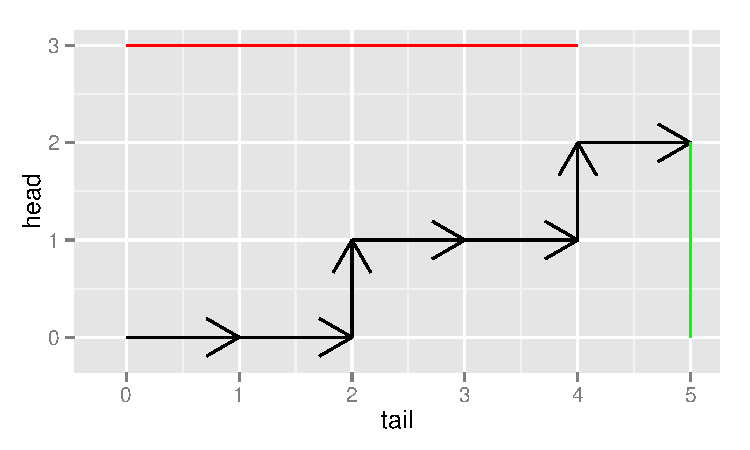
\includegraphics[width=\textwidth]{z-plot1.pdf}
\caption{
A hypothetical realization of the Bernoulli process.
}
\label{fig:z_plot}
\end{figure}

\section{Rotating the Z-Plot}


\bibliography{references}
\bibliographystyle{jss}

\end{document}
